\documentclass[11pt,aps,preprint,nofootinbib,superscriptaddress,tightenlines]{revtex4-2}
\usepackage{amsmath,amssymb,bm,mathtools,graphicx}
\usepackage{xcolor}
\definecolor{darkblue}{RGB}{0,0,160}
\usepackage[colorlinks=true,linkcolor=darkblue,citecolor=darkblue,urlcolor=darkblue]{hyperref}

\def\st{\begin{equation}}
\def\stp{\end{equation}}
\def\Eq#1{eq.~(\ref{#1})}
\def\Sect#1{Sect.~\ref{#1}}
\def\Fig#1{Fig.~\ref{#1}}
\newcommand{\avg}[1]{\langle #1\rangle}
\let\oldparagraph\paragraph
\renewcommand{\paragraph}{\par\bigskip\oldparagraph}

\begin{document}

\title{A moving fluid: equilibrium correlators at nonzero velocity}
\author{D.~Teaney}
\affiliation{Department of Physics and Astronomy, Stony Brook University,
Stony Brook, New York 11794, USA}
\date{\today}

\begin{abstract}
All runs so far were of a fluid at rest.  Here the fluid moves with a uniform velocity $v$
along $x$, $v=0$, $0.3$, $0.6$, $0.8$, at the same rest-frame entropy density.  The scheme is
started in equilibrium at the moving $\beta^\mu$, and the correlators of the energy and
momentum densities are measured for wave vectors along and across the flow, against
linearized hydrodynamics of the boosted fluid.  This note gives the plan, the changes to the
code, the predictions, and the results as they arrive.
\end{abstract}

\maketitle

%=============================================================================
\section{The state}
\label{sec:state}

A fluid with rest-frame entropy density $s_0$ and temperature $T_0$ (here $s_0=S_0=10^6$, so
$T_{\rm rel}=90.9$ as in all earlier runs) moving with velocity $\bm v=v\hat x$ has, in the lab,
\st
u^\mu=\gamma(1,v,0),\qquad
\beta^\mu=\frac{u^\mu}{T_0},\qquad \gamma=\frac{1}{\sqrt{1-v^2}} .
\stp
The densities the code carries (density frame) are the lab entropy density and the lab
energy and momentum densities,
\st
S=\gamma s_0,\qquad
\varepsilon\equiv T^{00}=w_0\gamma^2-p_0,\qquad
M_x\equiv T^{0x}=w_0\gamma^2v,
\label{densities}
\stp
with $w_0=e_0+p_0$ the rest-frame enthalpy.  For the conformal equation of state of the code,
$e=T^4$, $p=e/3$.  Each particle carries the entropy $s_a=\gamma s_0V$ ($V$ the lab volume per
particle): a boost raises the entropy per particle, so it does not push towards the wall of
\texttt{continuum\_limit.tex}.

\paragraph{The start.}  The uniform state \Eq{densities} is set on the hexagonal lattice, and
\texttt{equilibrium\_init!} draws the particle energies and momenta at the global $\beta^\mu$ whose
averages are these totals (\texttt{eqstart.tex}); it already handles $\bm\beta\ne0$.  A test at
$v=0.6$ and $0.8$ (box $0.6$) finds $\beta^\mu$ back with $v=0.601$, $0.800$ and the rest-frame
temperature to $10^{-4}$.

%=============================================================================
\section{What is measured}
\label{sec:measure}

The runs record the Fourier modes of the particle energies and momenta,
\st
E_{\bm k}=\sum_ae_a\,e^{-i\bm k\cdot\bm x_a},\qquad
\bm M_{\bm k}=\sum_a\bm m_a\,e^{-i\bm k\cdot\bm x_a},
\stp
for all box wave vectors with $kh\le1$.  Two directions are used:
\begin{itemize}
\item $\bm k\parallel\bm v$ ($\bm k=k\hat x$): the longitudinal momentum $M_x$ and the energy $E$
  carry the two sound modes, now Doppler shifted; the transverse momentum $M_y$ carries the
  shear mode, now advected.
\item $\bm k\perp\bm v$ ($\bm k=k\hat y$): $M_y$ is longitudinal (sound across the flow); $M_x$,
  the momentum along the flow, is transverse to $\bm k$ but mixes with $E$, because a change of
  the energy density at fixed velocity changes $M_x=w\gamma^2v$.
\end{itemize}
The correlators are complex, since the flow breaks $\bm k\to-\bm k$:
\st
C_{AB}(\bm k,\tau)=\frac{1}{NV}\avg{A_{\bm k}(t+\tau)\,B_{\bm k}^*(t)},\qquad A,B\in\{E,M_x,M_y\}.
\stp

\paragraph{Equal time.}  In equilibrium at $\beta^\mu$ the densities $U=(\varepsilon,M_x,M_y)$
fluctuate with the susceptibilities
\st
\chi_{ij}=\frac{\partial\avg{U_i}}{\partial\theta_j},\qquad
\theta=(-\beta^0,\beta^x,\beta^y),
\label{chi}
\stp
the second derivatives of $\log Z$ for the weight $e^{-\beta^0E+\bm\beta\cdot\bm M}$.  The particle
sums are white, so $C_{AB}(\bm k,0)=\chi_{AB}$ at every $k$.  The momentum susceptibilities grow
with $\gamma$: the fluctuations of a moving fluid are larger than $w_0T_0$.

\paragraph{Dynamics.}  For small $k$ linearized hydrodynamics gives
\st
\partial_t\delta U+i\,K(\bm k)\,\delta U=0,\qquad K(\bm k)=k_j\frac{\partial F_j}{\partial U},
\stp
with $F_j=(M_j,\,T^{jx},\,T^{jy})$ the ideal fluxes, $T^{ij}=w\gamma^2v^iv^j+p\,\delta^{ij}$,
differentiated numerically through the equation of state.  Then
\st
C(\bm k,\tau)=\sum_nP_n\,\chi\;e^{-i\omega_n\tau},
\stp
with $\omega_n$ and $P_n$ the eigenvalues and projectors of $K$.  The damping is added mode by
mode by boosting the rest-frame mode: a mode with rest-frame dispersion
$\omega'=\Omega(\bm k')-i\Gamma'(\bm k')$, with $\Gamma'=\nu k'^2$ (shear) or $\tfrac12\Gamma_sk'^2$ (sound,
$\Gamma_s=\tfrac43\nu$), $\nu=(\eta/s)/T_0$, has in the lab
\st
\omega=\omega_0-\frac{i\Gamma'}{\gamma\,(1+v\,\partial\Omega/\partial k'_x)},
\qquad \omega'=\gamma(\omega-vk_x),\quad k'_x=\gamma(k_x-v\omega),\quad k'_y=k_y .
\label{damp}
\stp
The simple cases:
\begin{center}
\begin{tabular}{lll}
\hline
mode & lab frequency & lab damping \\ \hline
shear, $\bm k\parallel\bm v$ & $vk$ (advected) & $\nu k^2/\gamma^3$ \\
shear, $\bm k\perp\bm v$ & $0$ & $\nu k^2/\gamma$ \\
sound, $\bm k\parallel\bm v$ & $k\,(v\pm c_s)/(1\pm vc_s)$ & from \Eq{damp} \\
sound, $\bm k\perp\bm v$ & $\pm k\,c_s\sqrt{(1-v^2)/(1-c_s^2v^2)}$ & from \Eq{damp} \\
\hline
\end{tabular}
\end{center}
The analysis code reproduces these limits (check before the runs): at $v=0$, $\chi_{xx}=wT$ and
$\chi_{EE}=T^2de/dT$ to $10^{-6}$; the ideal modes along the flow are $0.4138$, $0.8$, $0.9422$ (in units of
$k$) at $v=0.8$, across it $\pm0.3906$, as in the table; the susceptibilities grow as
\begin{center}
\begin{tabular}{lcccc}
\hline
$v$ & 0 & 0.3 & 0.6 & 0.8 \\ \hline
$\chi_{EE}/\chi_{EE}(0)$ & 1 & 1.26 & 2.66 & 7.59 \\
$\chi_{xx}/\chi_{xx}(0)$ & 1 & 1.67 & 5.47 & 19.4 \\
$\chi_{yy}/\chi_{yy}(0)$ & 1 & 1.05 & 1.25 & 1.67 \\
\hline
\end{tabular}
\end{center}
so the kinetic energy of the fluctuations about the mean flow, in the units $2VwT$ of the code, is
$\tfrac12(\chi_{xx}+\chi_{yy})\gamma/\chi_{xx}(0)$: $4.2$ at $v=0.6$, $17.6$ at $0.8$ (the smoke runs gave $4.0$, $17.3$).

These are the tests: the frequencies (advection, the relativistic addition of velocities, the
slower sound across the flow) and the dampings (time dilation, $\gamma^{-1}$ and $\gamma^{-3}$).

%=============================================================================
\section{Changes to the code}
\label{sec:code}

\begin{itemize}
\item \texttt{examples/stochrep\_equilibrium.jl}: \texttt{SR\_BOOST=v} sets the boosted uniform state
  \Eq{densities} (the rest-frame enthalpy $w_0$ from a rest-frame setup at $S_0$) before the
  equilibrium start; with a boost the energy modes $E_{\bm k}$ are recorded (\texttt{SR\_RECORD\_E=1}
  forces them at rest); the kinetic energy is measured about the mean flow; the run record
  (\texttt{.json}) has the boost, $\gamma$, the rest-frame and lab densities.
\item The physics code (ideal step, stochastic step, back map) is unchanged: the stochastic
  step already uses the comoving forms of its coefficients (\texttt{stochrep.tex}, ``A moving
  fluid'').
\item \texttt{examples/boost\_analysis.jl}: direction-resolved complex correlators, the
  susceptibilities \Eq{chi}, and the hydrodynamic predictions.
\end{itemize}

\paragraph{Time step.}  The time step of the code is set by $c_s$; signals now move at up to
$v_{\rm sig}=(v+c_s)/(1+vc_s)$ ($0.75$, $0.87$, $0.94$ at $v=0.3$, $0.6$, $0.8$).  The time step is
scaled by $c_s/v_{\rm sig}$: factors $0.8$, $0.66$, $0.6$; one set at $v=0.8$ runs at half of that.

%=============================================================================
\section{Runs}
\label{sec:runs}

Campaign \texttt{boost} (\texttt{nersc/campaign\_boost.txt}): $L=1.2$ ($kh\ge0.26$), $h/a=2$, $\eta/s=0.2$,
n-scheme, $t=300$, 16 runs at each $v=0$, $0.3$, $0.6$, $0.8$, and 4 at $v=0.8$ with $\Delta t/2$; two
nodes, packed (jobs 61156299, 61156300).  A larger box, $L=2.4$ ($kh\ge0.13$), 8 runs at $v=0$, $0.6$, $0.8$,
runs on a third node (61156353).  The long shear times ($\gamma^3/\nu k^2\approx75$ at $v=0.8$, $kh=0.26$) set $t=300$. 

%=============================================================================
\section{Results}
\label{sec:results}

\paragraph{The runs.}  The 68 runs at $L=1.2$ finished in 25--30 minutes per node (jobs 61156299,
61156300).  None broke; the stochastic step behaves as at rest (residual acceptance $0.83$--$0.84$, no
proposal reaches $|v|=1$ at these entropies).  The rest-frame temperature is held: $T_{\rm rel}=90.88$,
$90.88$, $90.87$, $90.86$ at $v=0$, $0.3$, $0.6$, $0.8$, and $\Delta H/H\le2\times10^{-3}$ by $t=300$.  The kinetic energy
of the fluctuations about the mean flow, in the units $2VwT$, is $1.00$, $1.46$, $4.49$, $19.3$, against the
predicted $1$, $1.45$, $4.2$, $17.6$ (\Sect{sec:measure}).  Errors below are jackknife over the 16 runs.

\paragraph{1. Equal time}, \Fig{fig:bstatic}.  $C_{AA}(\bm k,0)/\chi_{AA}$ at the smallest $k$ ($kh=0.26$):
\begin{center}
\begin{tabular}{lcccccc}
\hline
 & \multicolumn{3}{c}{$\bm k\parallel\bm v$} & \multicolumn{3}{c}{$\bm k\perp\bm v$} \\
$v$ & $E$ & $M_x$ & $M_y$ & $E$ & $M_x$ & $M_y$ \\ \hline
0 & $1.02(5)$ & $1.02(5)$ & $1.07(6)$ & $0.94(3)$ & $1.15(7)$ & $0.94(3)$ \\
0.3 & $0.93(5)$ & $0.90(6)$ & $1.00(5)$ & $1.11(5)$ & $1.04(4)$ & $1.13(6)$ \\
0.6 & $0.93(11)$ & $0.92(12)$ & $0.99(6)$ & $0.98(3)$ & $1.00(4)$ & $0.96(5)$ \\
0.8 & $0.90(12)$ & $0.89(12)$ & $0.96(11)$ & $0.99(6)$ & $1.01(6)$ & $0.94(6)$ \\
\hline
\end{tabular}
\end{center}
The fluctuations are those of the moving fluid, to within the errors, although $\chi_{xx}$ is 19 times
its rest value at $v=0.8$.  (Along the flow the values sit a little below 1 at every $v>0$, $1$--$2\sigma$;
the larger box will tell.)

\paragraph{2. The shear mode along the flow is advected}, \Fig{fig:bshear}.  $C_{yy}(k\hat x,\tau)$
oscillates at the advection frequency $vk$ inside the decaying envelope.  Fitting
$C\propto e^{-i\Omega\tau-\Gamma\tau}$ (\Fig{fig:bfit}):
\begin{center}
\begin{tabular}{lcccc}
\hline
$v$ & $\Omega/k$ & $\Gamma/(\nu k^2/\gamma^3)$, $\bm k\parallel\bm v$ & $\Gamma/(\nu k^2/\gamma)$, $\bm k\perp\bm v$ \\ \hline
0 & $0.002(1)$ & $0.84(12)$ & $1.04(12)$ \\
0.3 & $0.302(1)$ & $1.03(10)$ & $1.07(8)$ \\
0.6 & $0.598(1)$ & $0.99(12)$ & $0.90(8)$ \\
0.8 & $0.801(1)$ & $1.65(30)$ & $0.92(11)$ \\
\hline
\end{tabular}
\end{center}
The advection speed is $v$ to $10^{-3}$.  The damping follows time dilation: $\gamma^{-3}$ along the flow
(a factor $4.6$ at $v=0.8$) and $\gamma^{-1}$ across it, within the errors, except along the flow at $v=0.8$
($1.65\pm0.30$, $2\sigma$ high; there the decay time is $77$, a quarter of the run).

\paragraph{3. Sound along the flow}, \Fig{fig:bpar}.  $C_{xx}$ and $C_{EE}$ for $\bm k\parallel\bm v$ follow the
two Doppler-shifted sound modes, $(v\pm c_s)/(1\pm vc_s)=0.414$ and $0.942$ at $v=0.8$, with no adjustable
parameter: the curves lie on the predictions for twenty periods.

\paragraph{4. Across the flow}, \Fig{fig:bperp}.  $C_{yy}$ for $\bm k\perp\bm v$ is sound across the flow, slower
by $\sqrt{(1-v^2)/(1-c_s^2v^2)}$ ($0.68$ at $v=0.8$): the period grows as predicted.  $C_{xx}$ for $\bm k\perp\bm v$
is the shear mode of the momentum along the flow, mixed with sound through $\delta M_x=\delta w\,\gamma^2v$; the
mixture (the sound wiggles on the decaying shear) is reproduced.

\paragraph{So far.}  A fluid moving at up to $v=0.8$ is simulated in equilibrium, and its correlators
along and across the flow are those of boosted fluctuating hydrodynamics: susceptibilities, advection,
the relativistic addition of the sound speed, and the time dilation of the damping.  Open: the shear
damping along the flow at $v=0.8$; the larger box ($L=2.4$, $kh\ge0.13$) is running.

\begin{figure}[t]
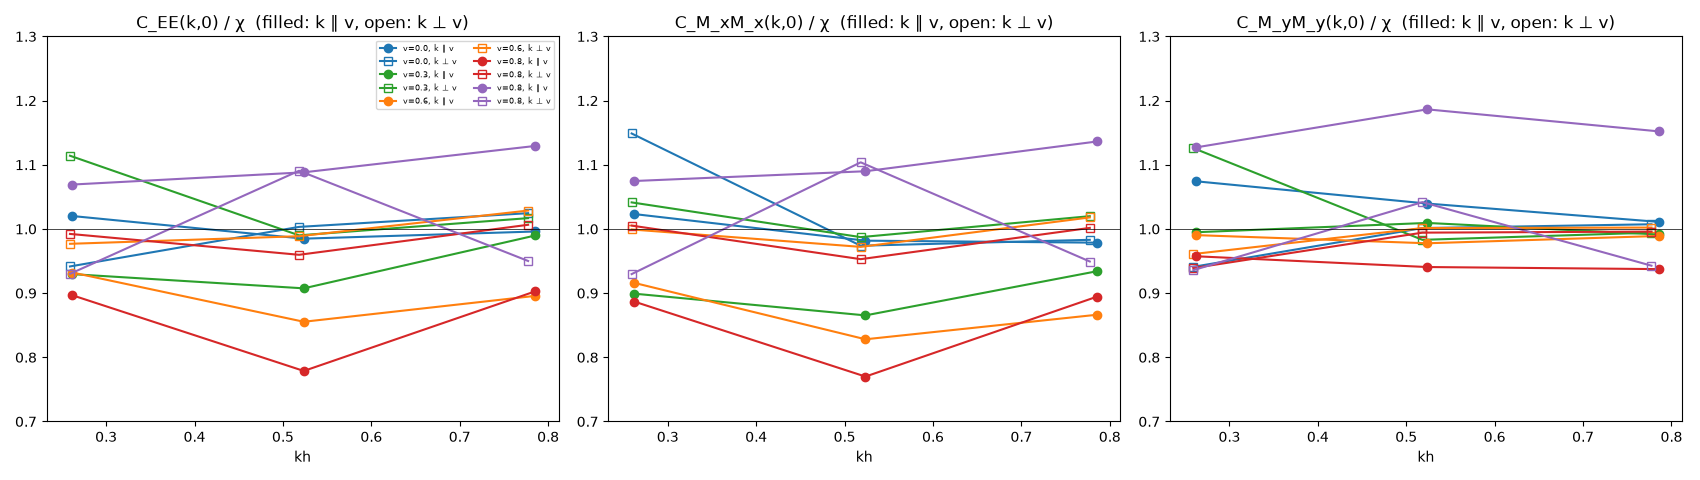
\includegraphics[width=\textwidth]{figs/boost_static.png}
\caption{Equal-time $C_{AA}(\bm k,0)/\chi_{AA}$ against $kh$ for $A=E$, $M_x$, $M_y$; filled: $\bm k\parallel\bm v$,
open: $\bm k\perp\bm v$; colour: $v$ (purple: $v=0.8$ at $\Delta t/2$, 4 runs).}
\label{fig:bstatic}
\end{figure}
\begin{figure}[t]
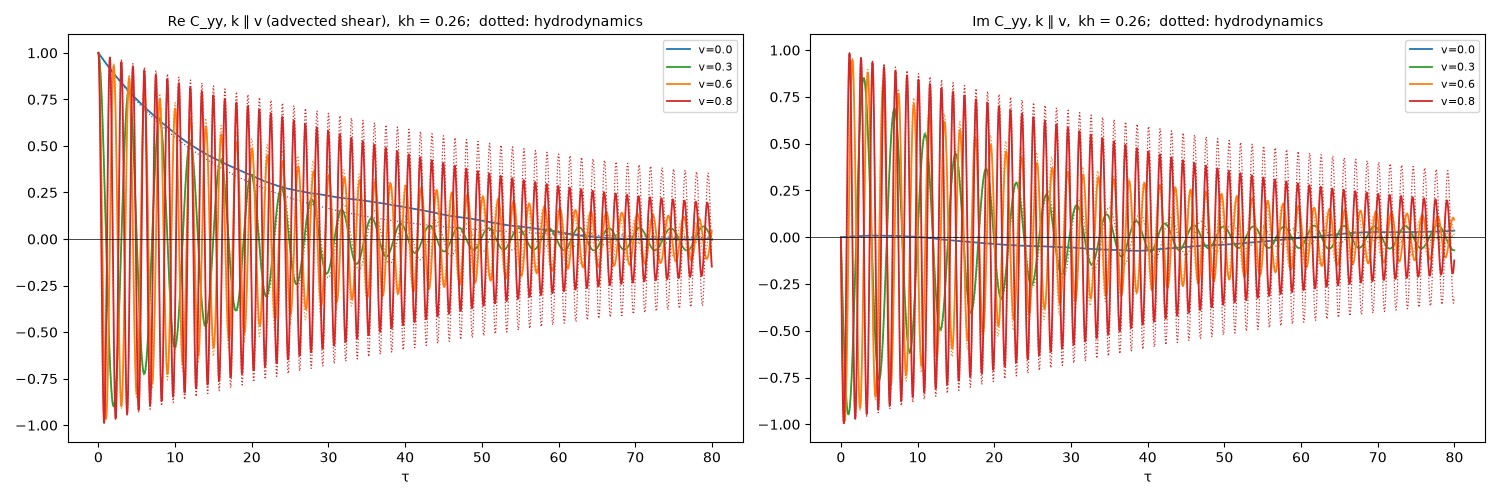
\includegraphics[width=\textwidth]{figs/boost_shear.png}
\caption{$\bm k\parallel\bm v$, $kh=0.26$: real and imaginary parts of $C_{yy}(\bm k,\tau)/C_{yy}(\bm k,0)$, the advected shear
mode; dotted: hydrodynamics (no fit).}
\label{fig:bshear}
\end{figure}
\begin{figure}[t]
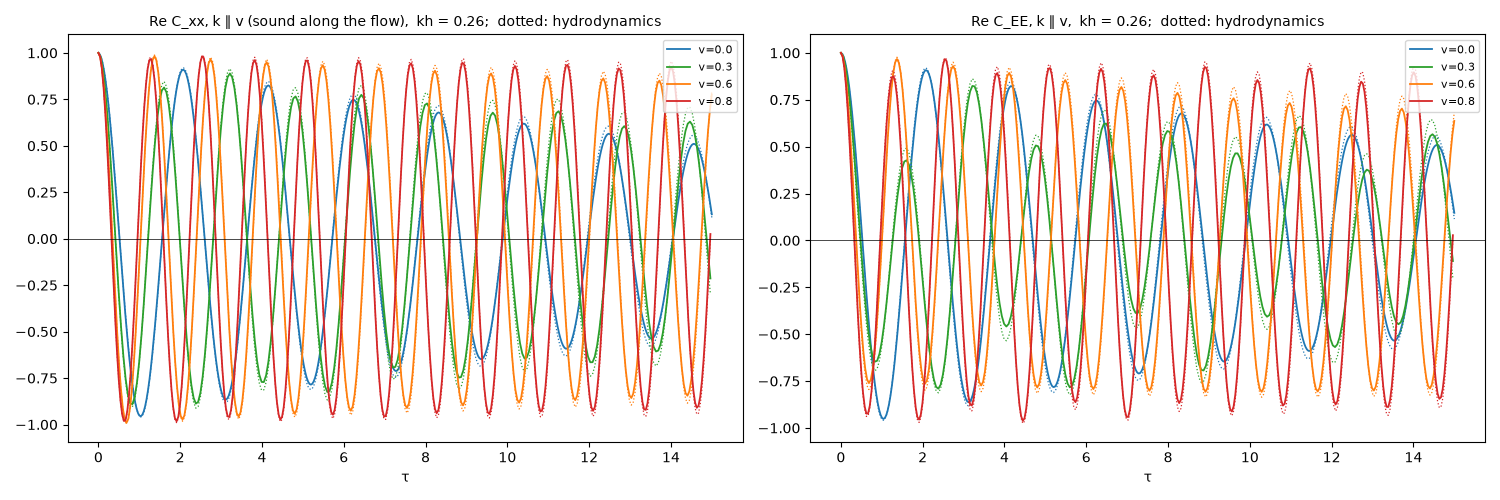
\includegraphics[width=\textwidth]{figs/boost_par.png}
\caption{$\bm k\parallel\bm v$, $kh=0.26$: $\mathrm{Re}\,C_{xx}$ and $\mathrm{Re}\,C_{EE}$ (normalized), the Doppler-shifted sound modes;
dotted: hydrodynamics.}
\label{fig:bpar}
\end{figure}
\begin{figure}[t]
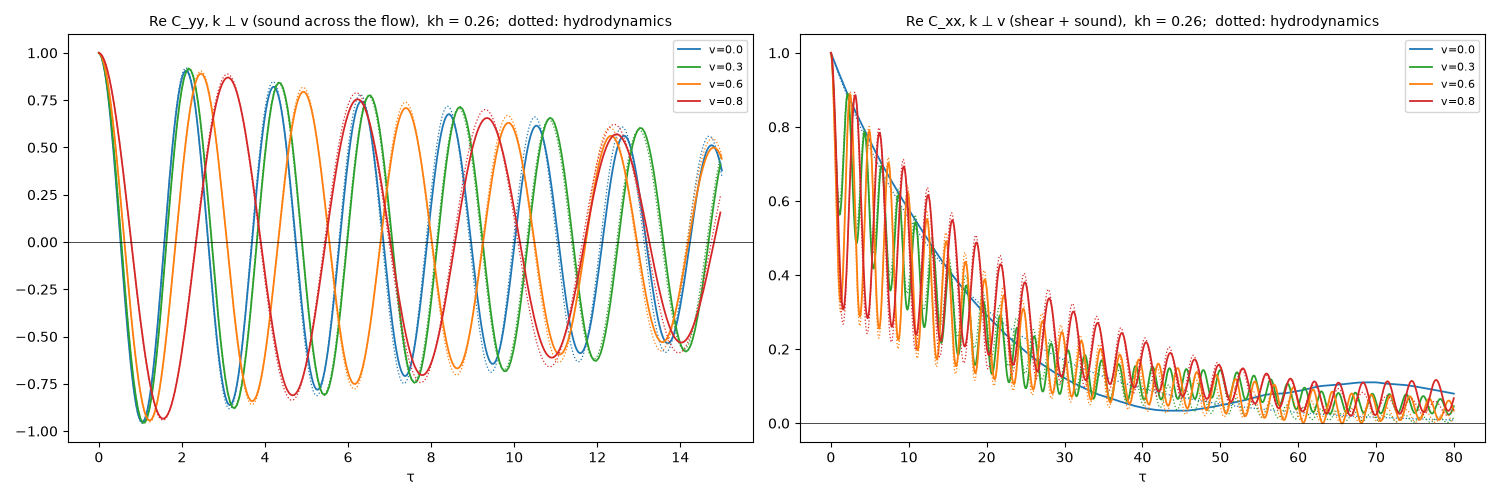
\includegraphics[width=\textwidth]{figs/boost_perp.png}
\caption{$\bm k\perp\bm v$, $kh=0.26$: $\mathrm{Re}\,C_{yy}$ (sound across the flow) and $\mathrm{Re}\,C_{xx}$ (shear of the momentum
along the flow, mixed with sound); dotted: hydrodynamics.}
\label{fig:bperp}
\end{figure}
\begin{figure}[t]
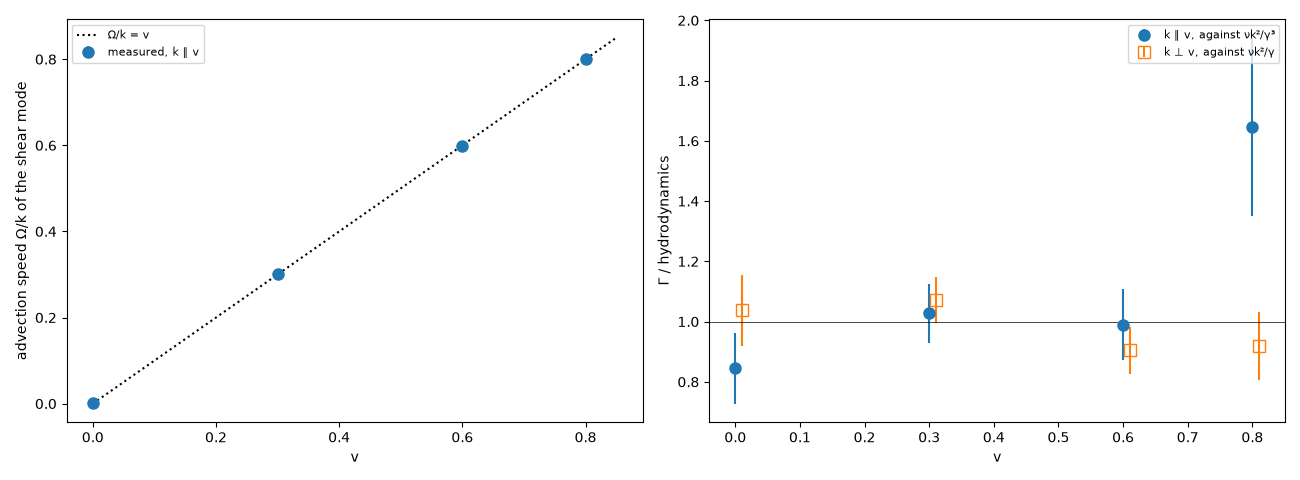
\includegraphics[width=\textwidth]{figs/boost_fit.png}
\caption{Fits of the shear modes at $kh=0.26$: advection speed $\Omega/k$ against $v$, and the damping
against $\nu k^2/\gamma^3$ ($\bm k\parallel\bm v$) and $\nu k^2/\gamma$ ($\bm k\perp\bm v$); jackknife errors.}
\label{fig:bfit}
\end{figure}

(The $L=2.4$ results are added when job 61156353 finishes.)

\end{document}
